% ===================================================================
% Arquivo: capitulos/parte-III-pilares/cap-10-perda-binaria.tex
% ===================================================================

\chapter{Funções de Perda}
\label{cap:perda-binaria}

Até agora foi visto o funcionamento da retropropagação, e como ela faz uso dos otimizadores, os quais funcionam como um barco, percorrendo a função de perda em busca de pontos de mínimos. Além disso, em seguida foram vistas diversas funções de ativação, começando pelas sigmoidais, depois pelas retificadoras, e por fim uma coletânea de diferentes funções. Contudo, está na hora de entender o outro lado da retropropagação: as funções de perda.

Para isso, esse capítulo busca explicar diversas funções de perda e suas aplicações, começando pelas funções para problemas de regressão, conhecendo as clássicas erro quadrático médio e erro absoluto médio, além da \textit{hubber loss}, uma função que busca unir o melhor dessas duas funções de perda. Seguindo adiante, são introduzidas as funções de perda para classificação binária, como a \textit{BCE}. Visto os problemas de classificação binária, é possível também conhecer os problemas de classifação multi com a \textit{categorical cross entropy}.

Mais adiante, está apresentado não funções, mas esquemas de como a perda pode ser medida para problemas como o de redes adversárias. Mas as perdas não são a única forma de medir como um modelo está performando, para isso, o final do capítulo é dedicado para explicar outros diferentes métodos de medir o desempenho do modelo que está sendo construído.

\section{A Intuição da Perda: Medindo o Erro do Modelo}

\section{Funções de Perda Para Regressão}

\subsection{Exemplo Ilustrativo: Jogando Dardos}

\subsection{Erro Quadrático Médio (Mean Squared Error - MSE)}


\begin{equacaodestaque}{Erro Quadrático Médio (MSE)}
    L_{\text{MSE}} = \frac{1}{N} \sum_{i=1}^{N} (y_i - \hat{y}_i)^2
    \label{eq:mse}
\end{equacaodestaque}

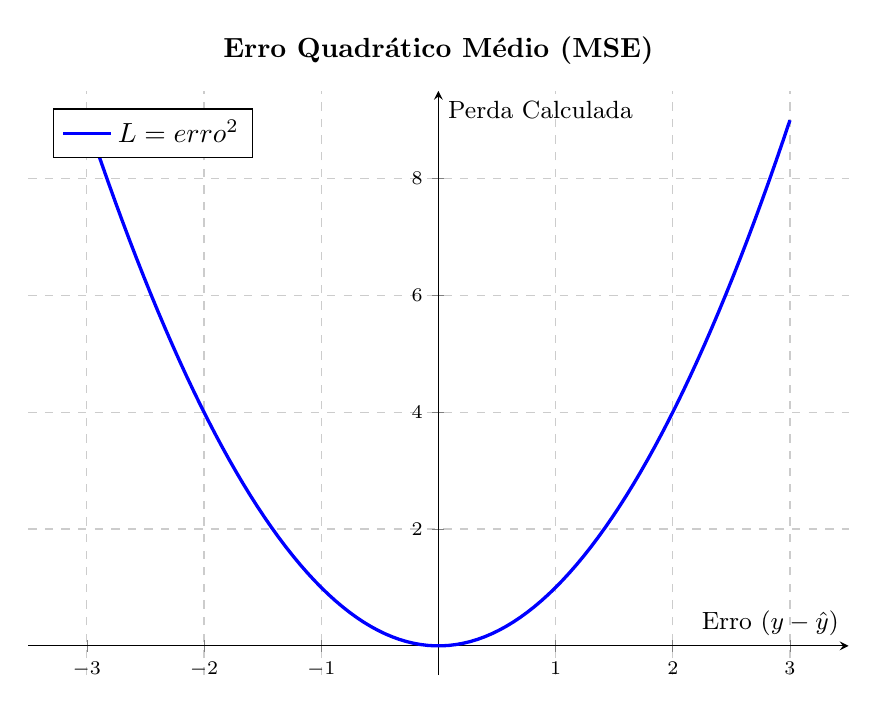
\begin{tikzpicture}
    \begin{axis}[
        title={Erro Quadrático Médio (MSE)},
        xlabel={Erro ($y - \hat{y}$)},
        ylabel={Perda Calculada},
        axis lines=middle,          % Eixos centrados em (0,0)
        grid=major,                 % Adiciona uma grade principal
        grid style={dashed, gray!40}, % Estilo da grade
        xmin=-3.5, xmax=3.5,        % Limites do eixo x
        ymin=-0.5, ymax=9.5,         % Limites do eixo y
        legend pos=north west,      % Posição da legenda
        width=12cm,                 % Largura do gráfico
        height=9cm,                 % Altura do gráfico
        title style={font=\bfseries},
        label style={font=\small},
        tick label style={font=\scriptsize}
    ]
        % Adiciona o gráfico da função x^2
        \addplot[
            domain=-3:3, 
            samples=100, 
            color=blue, 
            very thick
        ] {x^2};
        
        % Adiciona uma entrada na legenda
        \addlegendentry{$L = \text{erro}^2$}
    \end{axis}
\end{tikzpicture}

\begin{equacaodestaque}{Derivada do MSE}
    \frac{\partial L_{\text{MSE}}}{\partial \hat{y}_i} = \frac{2}{N}(\hat{y}_i - y_i)
    \label{eq:mse-derivada}
\end{equacaodestaque}


\subsection{Erro Absoluto Médio (Mean Absolute Error - MAE)}


\begin{equacaodestaque}{Erro Absoluto Médio (MAE)}
    L_{\text{MAE}} = \frac{1}{N} \sum_{i=1}^{N} |y_i - \hat{y}_i|
    \label{eq:mae}
\end{equacaodestaque}

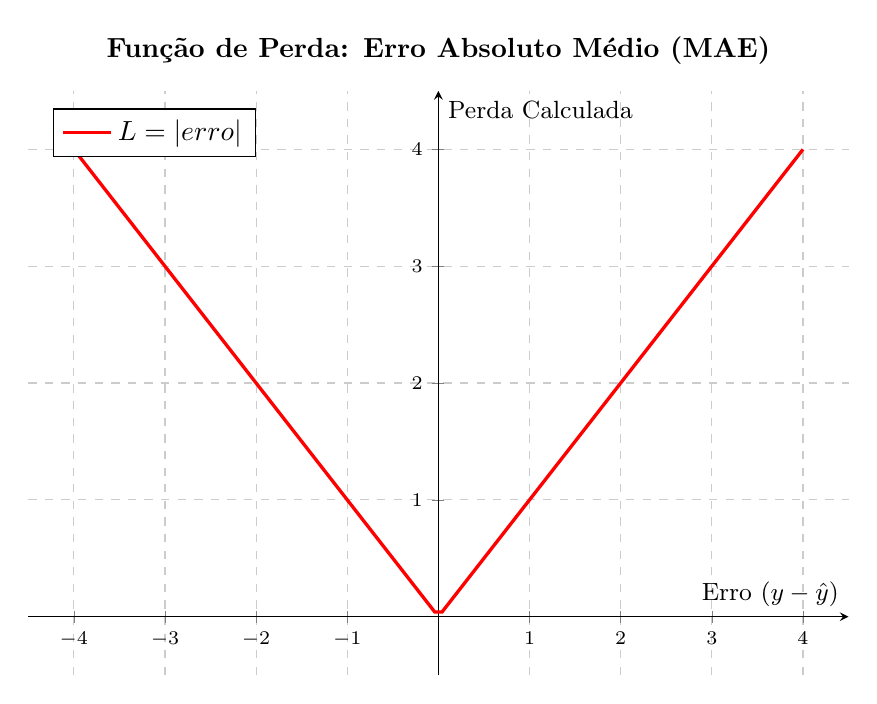
\begin{tikzpicture}
    \begin{axis}[
        title={Função de Perda: Erro Absoluto Médio (MAE)},
        xlabel={Erro ($y - \hat{y}$)},
        ylabel={Perda Calculada},
        axis lines=middle,          % Eixos centrados em (0,0)
        grid=major,                 % Adiciona uma grade principal
        grid style={dashed, gray!40}, % Estilo da grade
        xmin=-4.5, xmax=4.5,        % Limites do eixo x
        ymin=-0.5, ymax=4.5,         % Limites do eixo y
        legend pos=north west,      % Posição da legenda
        width=12cm,                 % Largura do gráfico
        height=9cm,                 % Altura do gráfico
        title style={font=\bfseries},
        label style={font=\small},
        tick label style={font=\scriptsize}
    ]
        % Adiciona o gráfico da função abs(x)
        \addplot[
            domain=-4:4, 
            samples=100, 
            color=red, 
            very thick
        ] {abs(x)};
        
        % Adiciona uma entrada na legenda
        \addlegendentry{$L = |\text{erro}|$}
    \end{axis}
\end{tikzpicture}

\begin{equacaodestaque}{Derivada do MAE}
    \frac{\partial L_{\text{MAE}}}{\partial \hat{y}_i} = \frac{1}{N} \cdot \text{sgn}(\hat{y}_i - y_i) = 
    \begin{cases} 
      +\frac{1}{N} & \text{se } \hat{y}_i > y_i \\
      -\frac{1}{N} & \text{se } \hat{y}_i < y_i \\
      0 & \text{se } \hat{y}_i = y_i
    \end{cases}
    \label{eq:mae-derivada}
\end{equacaodestaque}


\subsection{Huber Loss: O Melhor de Dois Mundos}


\begin{equacaodestaque}{Huber Loss}
    L_{\delta}(y, \hat{y}) = 
    \begin{cases} 
      \frac{1}{2}(y - \hat{y})^2 & \text{para } |y - \hat{y}| \le \delta \\
      \delta (|y - \hat{y}| - \frac{1}{2}\delta) & \text{caso contrário}
    \end{cases}
    \label{eq:huber-loss}
\end{equacaodestaque}

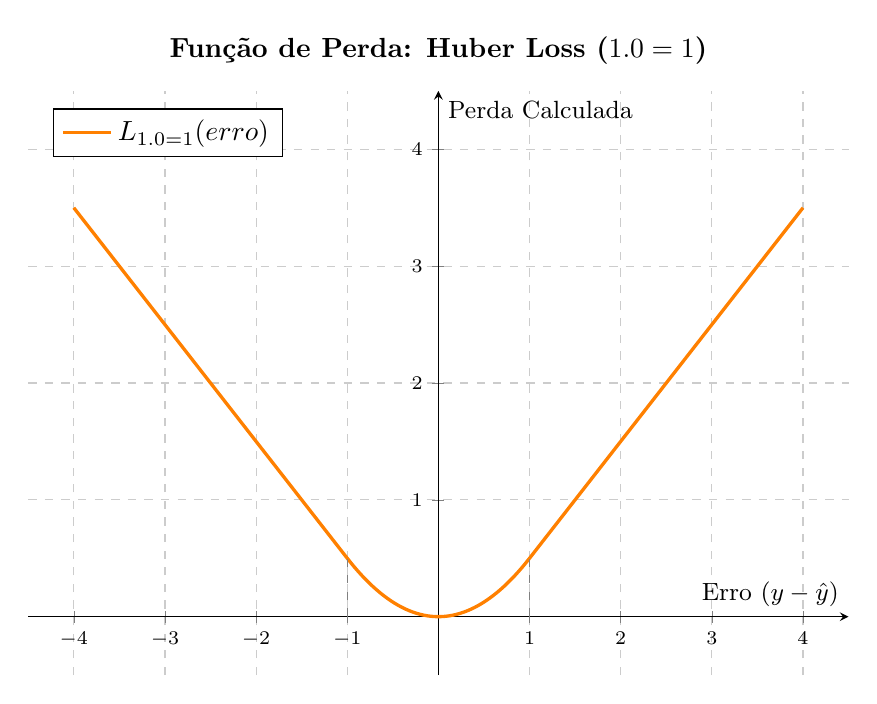
\begin{tikzpicture}
    \begin{axis}[
        title={Função de Perda: Huber Loss ($\delta=1$)},
        xlabel={Erro ($y - \hat{y}$)},
        ylabel={Perda Calculada},
        axis lines=middle,          % Eixos centrados em (0,0)
        grid=major,                 % Adiciona uma grade principal
        grid style={dashed, gray!40}, % Estilo da grade
        xmin=-4.5, xmax=4.5,        % Limites do eixo x
        ymin=-0.5, ymax=4.5,         % Limites do eixo y
        legend pos=north west,      % Posição da legenda
        width=12cm,                 % Largura do gráfico
        height=9cm,                 % Altura do gráfico
        title style={font=\bfseries},
        label style={font=\small},
        tick label style={font=\scriptsize}
    ]
        % Define o valor de delta
        \def\delta{1.0}

        % Adiciona o gráfico da função Huber usando uma expressão condicional
        % Se |x| <= delta, usa 0.5*x^2. Senão, usa delta*(|x| - 0.5*delta).
        \addplot[
            domain=-4:4, 
            samples=201, % Samples ímpares para incluir o ponto x=0
            color=orange, 
            very thick
        ] { abs(x) <= \delta ? 0.5*x^2 : \delta*(abs(x) - 0.5*\delta) };
        
        % Adiciona uma entrada na legenda
        \addlegendentry{$L_{\delta=1}(\text{erro})$}

        % Opcional: Adiciona linhas para mostrar a transição em delta
        \draw[dashed, gray] (axis cs:-\delta, 0) -- (axis cs:-\delta, {\delta*(\delta-0.5*\delta)});
        \draw[dashed, gray] (axis cs:\delta, 0) -- (axis cs:\delta, {\delta*(\delta-0.5*\delta)});

    \end{axis}
\end{tikzpicture}

\begin{equacaodestaque}{Derivada da Huber Loss}
    \frac{\partial L_{\delta}}{\partial \hat{y}} = 
    \begin{cases} 
      \hat{y} - y & \text{para } |\hat{y} - y| \le \delta \\
      \delta \cdot \text{sgn}(\hat{y} - y) & \text{caso contrário}
    \end{cases}
    \label{eq:huber-loss-derivada}
\end{equacaodestaque}

\section{Funções de Perda para Classificação Binária}

\subsection{Entropia Cruzada Binária (Binary Cross-Entropy): A função de perda padrão}

\begin{equacaodestaque}{Entropia Cruzada Binária}
    L(y, \hat{y}) = -[y \log(\hat{y}) + (1 - y) \log(1 - \hat{y})]
    \label{eq:binary-cross-entropy}
\end{equacaodestaque}

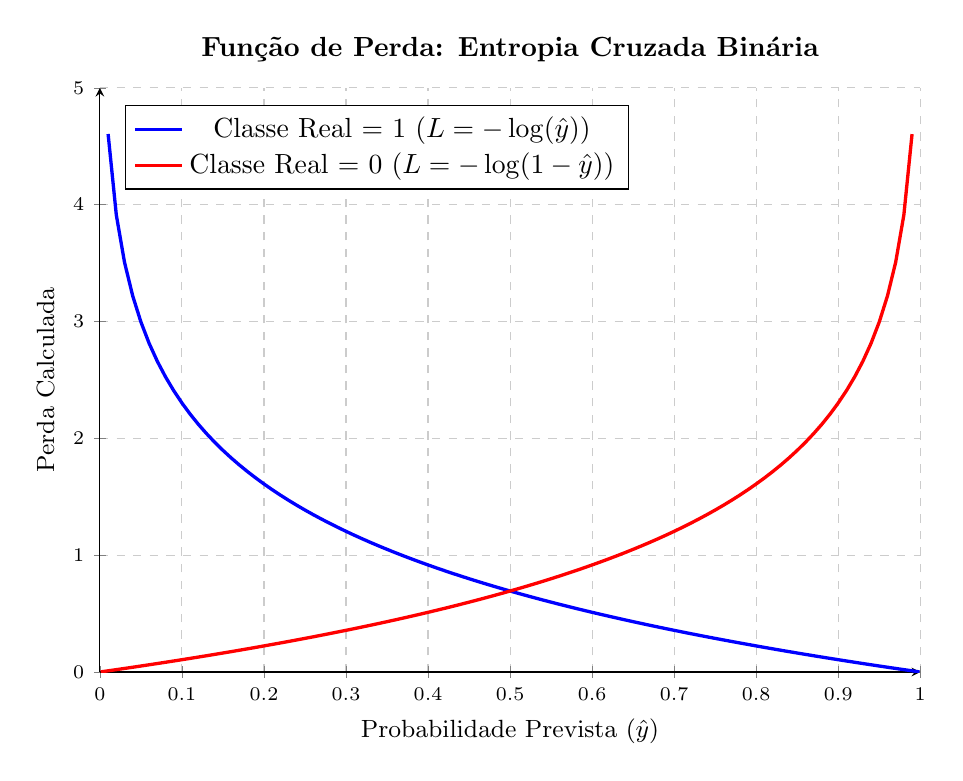
\begin{tikzpicture}
    \begin{axis}[
        title={Função de Perda: Entropia Cruzada Binária},
        xlabel={Probabilidade Prevista ($\hat{y}$)},
        ylabel={Perda Calculada},
        axis lines=left,              % Eixos no canto inferior esquerdo
        grid=major,                   % Adiciona uma grade principal
        grid style={dashed, gray!40},   % Estilo da grade
        xmin=0, xmax=1,               % Limites do eixo x
        ymin=0, ymax=5,               % Limites do eixo y
        legend pos=north west,      % Posição da legenda
        width=12cm,                   % Largura do gráfico
        height=9cm,                   % Altura do gráfico
        title style={font=\bfseries},
        label style={font=\small},
        tick label style={font=\scriptsize}
    ]
        % Curva para a classe real y=1
        \addplot[
            domain=0.01:0.999, % Domínio para evitar log(0)
            samples=100,
            color=blue,
            very thick
        ] {-ln(x)};
        \addlegendentry{Classe Real = 1 ($L = -\log(\hat{y})$)}

        % Curva para a classe real y=0
        \addplot[
            domain=0.001:0.99, % Domínio para evitar log(0)
            samples=100,
            color=red,
            very thick
        ] {-ln(1-x)};
        \addlegendentry{Classe Real = 0 ($L = -\log(1-\hat{y})$)}
        
    \end{axis}
\end{tikzpicture}

\begin{equacaodestaque}{Derivada da Entropia Cruzada Binária}
    \frac{\partial L}{\partial \hat{y}} = \frac{\hat{y} - y}{\hat{y}(1 - \hat{y})}
    \label{eq:binary-cross-entropy-derivada}
\end{equacaodestaque}

\subsection{Perda Hinge (Hinge Loss)}

\begin{equacaodestaque}{Hinge Loss}
    L(y, f(x)) = \max(0, 1 - y \cdot f(x))
    \label{eq:hinge-loss}
\end{equacaodestaque}

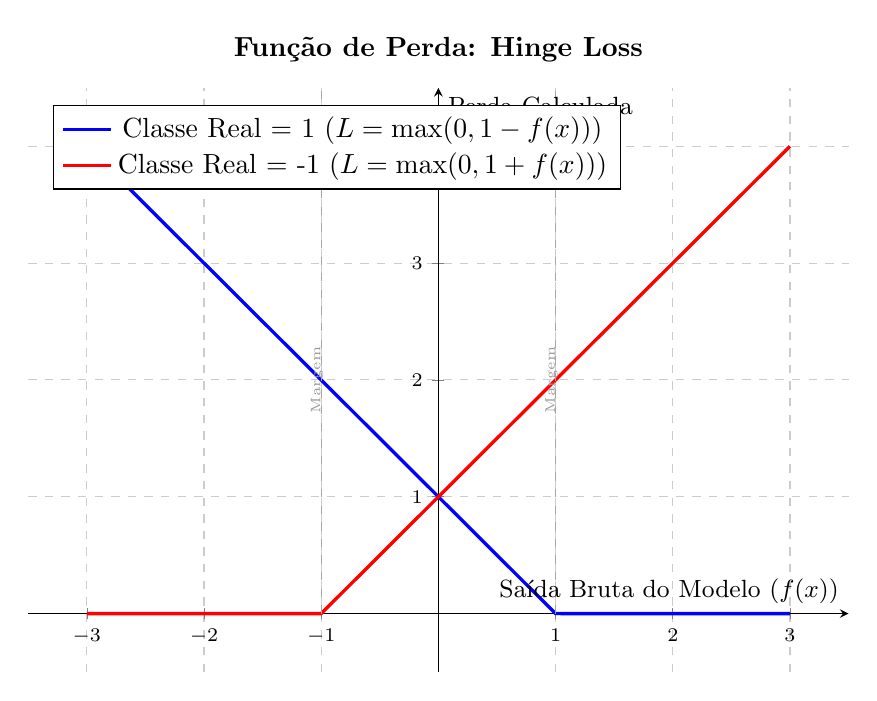
\begin{tikzpicture}
    \begin{axis}[
        title={Função de Perda: Hinge Loss},
        xlabel={Saída Bruta do Modelo ($f(x)$)},
        ylabel={Perda Calculada},
        axis lines=middle,          % Eixos centrados em (0,0)
        grid=major,                 % Adiciona uma grade principal
        grid style={dashed, gray!40}, % Estilo da grade
        xmin=-3.5, xmax=3.5,        % Limites do eixo x
        ymin=-0.5, ymax=4.5,         % Limites do eixo y
        legend pos=north west,      % Posição da legenda
        width=12cm,                 % Largura do gráfico
        height=9cm,                 % Altura do gráfico
        title style={font=\bfseries},
        label style={font=\small},
        tick label style={font=\scriptsize}
    ]
        % Curva para a classe real y=+1
        \addplot[
            domain=-3:3, 
            samples=100, 
            color=blue, 
            very thick
        ] {max(0, 1-x)};
        \addlegendentry{Classe Real = 1 ($L=\max(0, 1-f(x))$)}

        % Curva para a classe real y=-1
        \addplot[
            domain=-3:3, 
            samples=100, 
            color=red, 
            very thick
        ] {max(0, 1+x)};
        \addlegendentry{Classe Real = -1 ($L=\max(0, 1+f(x))$)}
        
        % Opcional: Linhas tracejadas para marcar as margens
        \draw[dashed, gray!70] (axis cs:1, 0) -- (axis cs:1, 4.5);
        \draw[dashed, gray!70] (axis cs:-1, 0) -- (axis cs:-1, 4.5);
        \node[above, gray!80, font=\tiny, rotate=90] at (axis cs:1.1, 2) {Margem};
        \node[above, gray!80, font=\tiny, rotate=90] at (axis cs:-0.9, 2) {Margem};
        
    \end{axis}
\end{tikzpicture}

\begin{equacaodestaque}{Derivada da Hinge Loss}
    \frac{\partial L}{\partial f(x)} = 
    \begin{cases} 
      -y & \text{se } y \cdot f(x) < 1 \\
      0 & \text{se } y \cdot f(x) \ge 1
    \end{cases}
    \label{eq:hinge-loss-derivada}
\end{equacaodestaque}

\section{Funções de Perda para Classificação Multilabel}

\subsection{Entropia Cruzada Categórica (Categorical Cross-Entropy)} 

\begin{equacaodestaque}{Entropia Cruzada Categórica}
    L(y, \hat{y}) = - \sum_{c=1}^{C} y_c \log(\hat{y}_c)
    \label{eq:categorical-cross-entropy}
\end{equacaodestaque}

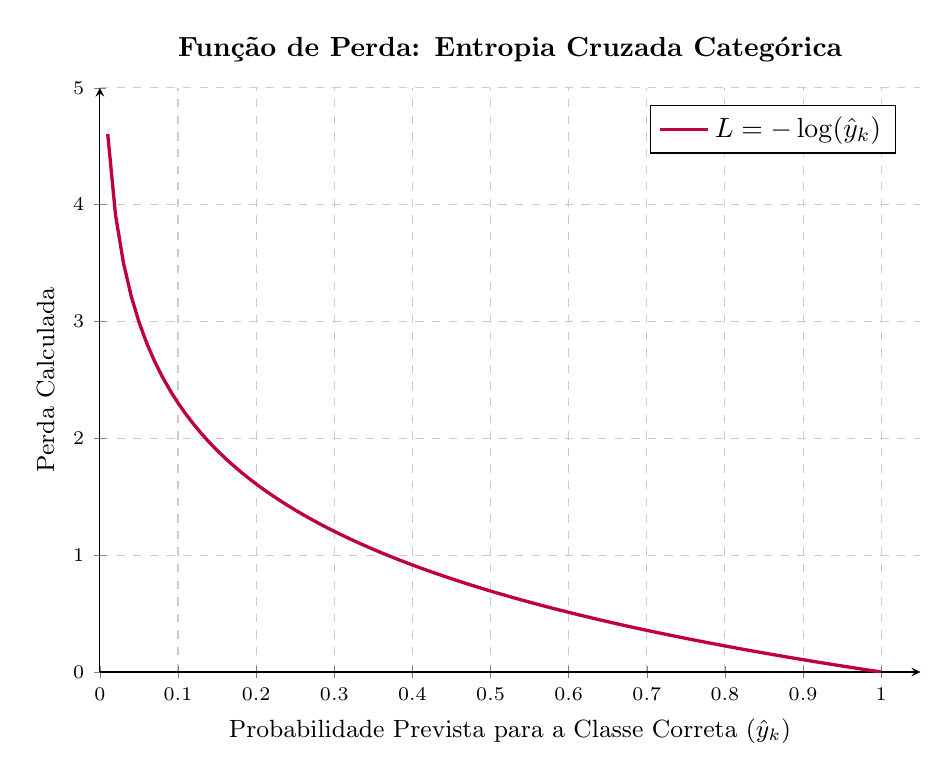
\begin{tikzpicture}
    \begin{axis}[
        title={Função de Perda: Entropia Cruzada Categórica},
        xlabel={Probabilidade Prevista para a Classe Correta ($\hat{y}_k$)},
        ylabel={Perda Calculada},
        axis lines=left,              % Eixos no canto inferior esquerdo
        grid=major,                   % Adiciona uma grade principal
        grid style={dashed, gray!40},   % Estilo da grade
        xmin=0, xmax=1.05,            % Limites do eixo x
        ymin=0, ymax=5,               % Limites do eixo y
        legend pos=north east,        % Posição da legenda
        width=12cm,                   % Largura do gráfico
        height=9cm,                   % Altura do gráfico
        title style={font=\bfseries},
        label style={font=\small},
        tick label style={font=\scriptsize}
    ]
        % Plota a função -log(y_k_hat)
        \addplot[
            domain=0.01:1, % Domínio para evitar log(0)
            samples=100,
            color=purple,
            very thick
        ] {-ln(x)};
        
        \addlegendentry{$L = -\log(\hat{y}_k)$}
        
    \end{axis}
\end{tikzpicture}

\begin{equacaodestaque}{Derivada da Entropia Cruzada Categórica}
    \frac{\partial L}{\partial z_i} = \hat{y}_i - y_i
    \label{eq:category-cross-entropy-derivada}
\end{equacaodestaque}

\subsection{Entropia Cruzada Categórica Esparsa (Sparse Categorical Cross-Entropy)}

\begin{equacaodestaque}{Entropia Cruzada Categórica Esparsa}
    L_i = - \log(\hat{y}_{i, y_i})
    \label{eq:sparse-categorical-cross-entropy}
\end{equacaodestaque}

\begin{equacaodestaque}{Derivada da Entropia Cruzada Categórica Esparsa}
    \frac{\partial L_i}{\partial z_{i,k}} = \hat{y}_{i,k} - y_{i,k}
    \label{eq:sparse-categorical-cross-entropy-derivada}
\end{equacaodestaque}

\section{Funções de Perda Avançadas}

\subsection{Perda para Classificação Multirrótulo (Multilabel)}

\begin{equacaodestaque}{Perda para Classificação Multirrótulo}
    \mathcal{L}_{\text{multilabel}} = - \frac{1}{C} \sum_{c=1}^{C} \left[ y_c \log(\hat{y}_c) + (1 - y_c) \log(1 - \hat{y}_c) \right]
    \label{eq:multilabel-loss}
\end{equacaodestaque}

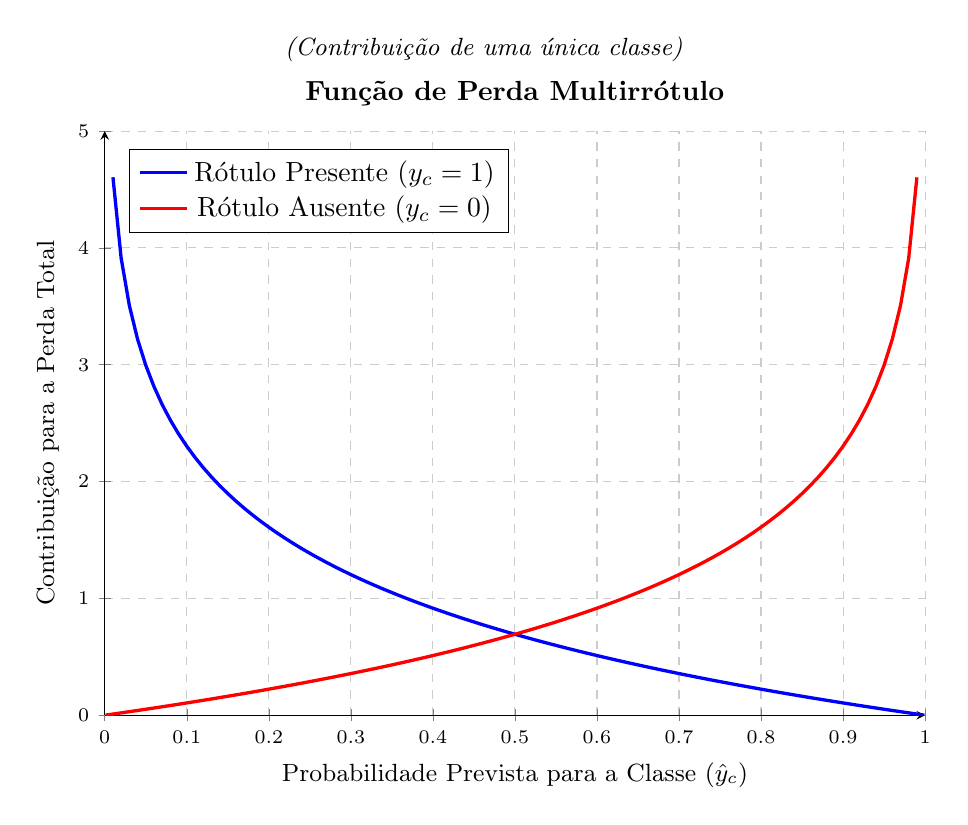
\begin{tikzpicture}
    \begin{axis}[
        title={Função de Perda Multirrótulo},
        % A chave "name=plot" foi removida daqui
        title style={font=\bfseries},
        xlabel={Probabilidade Prevista para a Classe ($ \hat{y}_c $)},
        ylabel={Contribuição para a Perda Total},
        axis lines=left,
        grid=major,
        grid style={dashed, gray!40},
        xmin=0, xmax=1,
        ymin=0, ymax=5,
        legend pos=north west,
        width=12cm,
        height=9cm,
        label style={font=\small},
        tick label style={font=\scriptsize}
    ]
        % Curva para quando o rótulo está presente (y_c = 1)
        \addplot[
            domain=0.01:0.999, 
            samples=100,
            color=blue,
            very thick
        ] {-ln(x)};
        \addlegendentry{Rótulo Presente ($y_c=1$)}

        % Curva para quando o rótulo está ausente (y_c = 0)
        \addplot[
            domain=0.001:0.99,
            samples=100,
            color=red,
            very thick
        ] {-ln(1-x)};
        \addlegendentry{Rótulo Ausente ($y_c=0$)}
        
    \end{axis} % --- O AMBIENTE AXIS TERMINA AQUI ---

    % --- NOVO NÓ PARA O SUBTÍTULO ---
    % Posicionado acima do centro da "caixa" do gráfico que acabamos de desenhar
    \node[anchor=south, font=\small\itshape] at (current bounding box.north) 
    {(Contribuição de uma única classe)};

\end{tikzpicture}

\begin{equacaodestaque}{Derivada da Perda Multirrótulo}
    \frac{\partial \mathcal{L}_{\text{multilabel}}}{\partial z_c} = \frac{1}{C}(\hat{y}_c - y_c)
    \label{eq:multilabel-loss-derivada}
\end{equacaodestaque}

\subsection{Perdas para Ranking e Aprendizado de Métricas}

\subsubsection{Triplet Loss (Perda Tripla)}

\begin{equacaodestaque}{Triplet Loss}
    \mathcal{L}(a, p, n) = \max \left( \| f(a) - f(p) \|^2 - \| f(a) - f(n) \|^2 + \alpha, 0 \right)
    \label{eq:triplet-loss}
\end{equacaodestaque}

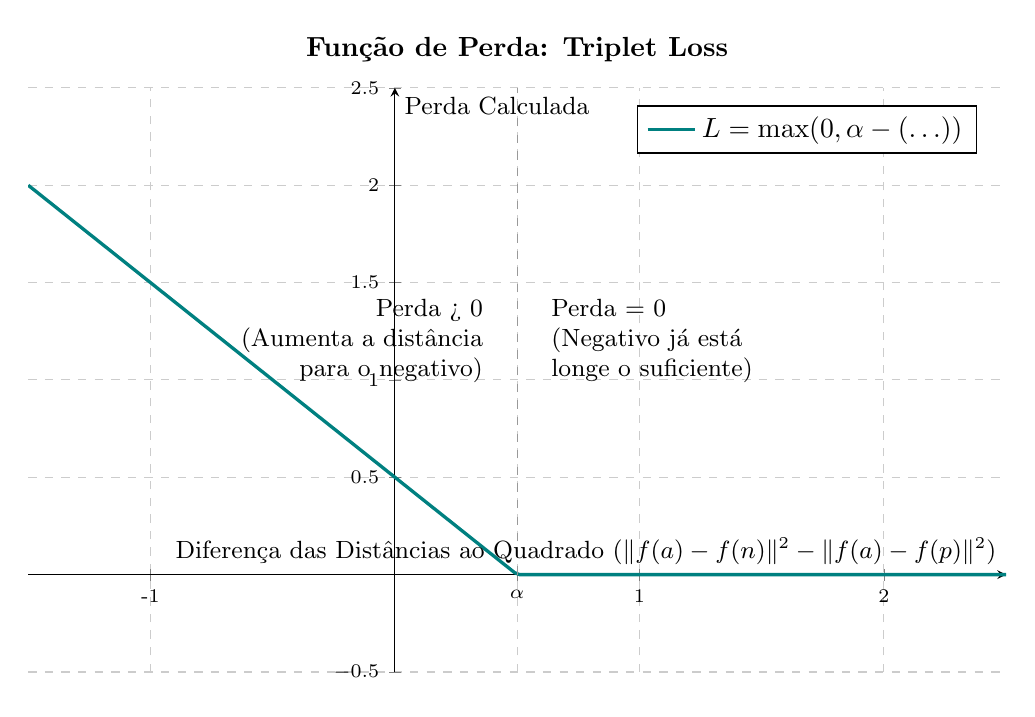
\begin{tikzpicture}
    \begin{axis}[
        title={Função de Perda: Triplet Loss},
        xlabel={Diferença das Distâncias ao Quadrado ($\|f(a)-f(n)\|^2 - \|f(a)-f(p)\|^2$)},
        ylabel={Perda Calculada},
        axis lines=middle,
        grid=major,
        grid style={dashed, gray!40},
        xmin=-1.5, xmax=2.5,
        ymin=-0.5, ymax=2.5,
        legend pos=north east,
        width=14cm, % Gráfico mais largo para o rótulo do eixo x
        height=9cm,
        title style={font=\bfseries},
        label style={font=\small},
        tick label style={font=\scriptsize},
        % Adiciona um 'tick' customizado para marcar a margem alpha
        xtick={-1, 0, 0.5, 1, 2},
        xticklabels={-1, 0, $\alpha$, 1, 2}
    ]
        % Define o valor da margem alpha
        \def\margin{0.5}

        % Plota a função max(0, alpha - x)
        % Onde x é a "diferença das distâncias" do eixo horizontal
        \addplot[
            domain=-1.5:2.5,
            samples=200,
            color=teal, % Uma nova cor para esta função
            very thick
        ] {max(0, \margin - x)};
        
        \addlegendentry{$L = \max(0, \alpha - (\dots))$}

        % Linha vertical para marcar onde a perda começa (na margem)
        \draw[dashed, gray!80] (axis cs:\margin, 0) -- (axis cs:\margin, 2.5);

        % Anotações para explicar as regiões do gráfico
        \node[anchor=west, align=left, font=\small] at (axis cs: \margin+0.1, 1.2) {Perda = 0 \\ (Negativo já está \\ longe o suficiente)};
        \node[anchor=east, align=right, font=\small] at (axis cs: \margin-0.1, 1.2) {Perda > 0 \\ (Aumenta a distância \\ para o negativo)};
        
    \end{axis}
\end{tikzpicture}

\subsubsection{Contrastive Loss (Perda Contrastiva)}

\begin{equacaodestaque}{Perda Composta (Conceitual)}
    \mathcal{L}_{\text{total}} = \lambda_{\text{reg}} \mathcal{L}_{\text{regressão}} + \mathcal{L}_{\text{classificação}}
    \label{eq:composite-loss}
\end{equacaodestaque}

\begin{tikzpicture}[
    node distance=1.7cm and 1.5cm,
    % Estilos dos blocos
    bloco/.style={
        rectangle, draw, thick, rounded corners=3mm,
        fill=blue!10, text centered, minimum height=1.2cm,
        text width=3.5cm, drop shadow={opacity=0.4}
    },
    saida/.style={
        rectangle, draw, thick, rounded corners=3mm,
        text centered, minimum height=1cm, text width=4.2cm
    },
    perda/.style={
        ellipse, draw, thick, fill=orange!20,
        text centered, minimum height=1.2cm, text width=3.2cm,
        drop shadow={opacity=0.4}
    },
    soma/.style={
        circle, draw, thick, fill=gray!20, minimum size=1cm,
        drop shadow={opacity=0.4}
    },
    final/.style={
        rectangle, draw, very thick, rounded corners=3mm,
        fill=green!20, text centered, minimum height=1.2cm, text width=3cm,
        drop shadow={opacity=0.4}
    },
    % Estilo das setas
    seta/.style={draw, -{Stealth[length=2.5mm]}, thick}
]

    % --- Nós do Diagrama ---

    % Entrada e Modelo
    \node[bloco] (input) {Imagem de Entrada};
    \node[bloco, below=of input] (model) {Rede Neural (Modelo)};

    % Saídas do Modelo
    \node[saida, fill=cyan!20, below left=1.2cm and -1.5cm of model] (out_class) {Saída de Classificação (Probabilidades)};
    \node[saida, fill=yellow!20, below right=1.2cm and -1.5cm of model] (out_reg) {Saída de Regressão (Coordenadas)};

    % Funções de Perda
    \node[perda, below=of out_class] (loss_class) {$\mathcal{L}_{\text{classificação}}$};
    \node[perda, below=of out_reg] (loss_reg) {$\mathcal{L}_{\text{regressão}}$};

    % Soma Ponderada
    \node[soma, below=2.2cm of model] (summation) {$\boldsymbol{+}$};

    % Perda Total
    \node[final, below=of summation] (total_loss) {$\mathcal{L}_{\text{total}}$};


    % --- Conexões (Setas) ---

    \path[seta] (input) -- (model);
    \path[seta] (model.south) |- (out_class.north);
    \path[seta] (model.south) |- (out_reg.north);

    \path[seta] (out_class) -- node[midway, right, font=\tiny] {vs. Rótulos Reais} (loss_class);
    \path[seta] (out_reg) -- node[midway, right, font=\tiny] {vs. Coordenadas Reais} (loss_reg);

    % Setas para a soma
    \path[seta] (loss_class.south) .. controls +(south:1cm) and +(west:1cm) .. (summation.west);
    \path[seta] (loss_reg.south) .. controls +(south:1cm) and +(east:1cm) .. node[midway, below right, pos=0.4] {$\times \lambda_{\text{reg}}$} (summation.east);

    % Seta final
    \path[seta, very thick, green!50!black] (summation) -- node[midway, right] {Para a Retropropagação} (total_loss);

\end{tikzpicture}

\begin{equacaodestaque}{Função de Valor de uma GAN (Minimax)}
    \min_{G} \max_{D} V(D, G) = \mathbb{E}_{x \sim p_{\text{data}}(x)}[\log D(x)] + \mathbb{E}_{z \sim p_{z}(z)}[\log(1 - D(G(z)))]
    \label{eq:gan-loss}
\end{equacaodestaque}

\begin{tikzpicture}[
    node distance=1.5cm and 2cm,
    % Estilos dos blocos
    gerador/.style={
        rectangle, draw, thick, rounded corners=3mm, fill=green!15, text centered,
        minimum height=1.5cm, text width=3.5cm, drop shadow={opacity=0.4}
    },
    discriminador/.style={
        rectangle, draw, thick, rounded corners=3mm, fill=red!15, text centered,
        minimum height=1.5cm, text width=3.5cm, drop shadow={opacity=0.4}
    },
    dados/.style={
        cylinder, shape border rotate=90, draw, thick, fill=gray!20, text centered,
        minimum height=1.5cm, text width=3cm, drop shadow={opacity=0.4}
    },
    ruido/.style={
        cloud, draw, thick, cloud puffs=10, fill=blue!10, aspect=1.5,
        text centered, minimum height=1.5cm, text width=2.5cm, drop shadow={opacity=0.4}
    },
    decisao/.style={
        ellipse, draw, thick, fill=orange!20, text centered,
        minimum height=1cm, text width=3.5cm, drop shadow={opacity=0.4}
    },
    % Estilo das setas
    seta/.style={draw, -{Stealth[length=2.5mm]}, thick},
    seta_feedback/.style={draw, -{Stealth[length=2.5mm]}, very thick, dashed}
]

    % --- Nós do Diagrama ---
    \node[ruido] (noise) {Vetor de Ruído ($z$)};
    \node[gerador, right=of noise] (generator) {Gerador (G)};
    \node[dados, below=of noise] (real_data) {Imagens Reais ($x$)};
    
    \node (fake_image_label) [below=0.7cm of generator] {Imagem Falsa $G(z)$};
    
    \node[discriminador, below=2cm of generator] (discriminator) {Discriminador (D)};
    
    \node[decisao, below=of discriminator] (decision) {Decisão: Real ou Falso?};

    % --- Setas de Fluxo de Dados ---
    \path[seta] (noise) -- (generator);
    \path[seta] (generator) -- (fake_image_label.north);
    
    \path[seta, green!50!black] (fake_image_label.south) -- (discriminator.north);
    \path[seta, red!50!black] (real_data) -- (discriminator.west);

    \path[seta] (discriminator) -- (decision);

    % --- Setas de Retropropagação (Feedback) ---
    % Objetivo do Discriminador: Maximizar V (acertar a classificação)
    \draw[seta_feedback, red!50!black] (decision.south) 
        to[bend right=60] 
        node[midway, fill=white, rounded corners=2pt, inner sep=2pt, font=\small] 
        {Atualizar D para $\max V(D,G)$ \\ (Aprende a diferenciar)} 
        (discriminator.south);
    
    % Objetivo do Gerador: Minimizar V (enganar o discriminador)
    \draw[seta_feedback, green!50!black] (decision.east) 
        to[bend left=70] 
        node[midway, fill=white, rounded corners=2pt, inner sep=2pt, font=\small] 
        {Atualizar G para $\min V(D,G)$ \\ (Aprende a enganar)} 
        (generator.east);
        
\end{tikzpicture}

\section{Outras Métricas de Avaliação}

\subsection{Acurácia}

\begin{equacaodestaque}{Acurácia}
    \text{Acurácia} = \frac{VP + VN}{VP + VN + FP + FN}
    \label{eq:acuracia}
\end{equacaodestaque}

\subsection{Precisão}

\begin{equacaodestaque}{Precisão (Precision)}
    \text{Precisão} = \frac{VP}{VP + FP}
    \label{eq:precisao}
\end{equacaodestaque}

\subsection{Revocação ou Sensibilidade}

\begin{equacaodestaque}{Revocação (Recall) ou Sensibilidade}
    \text{Revocação} = \frac{VP}{VP + FN}
    \label{eq:revocacao}
\end{equacaodestaque}

\subsection{F1-Score}

\begin{equacaodestaque}{F1-Score}
    \text{F1-Score} = 2 \times \frac{\text{Precisão} \times \text{Revocação}}{\text{Precisão} + \text{Revocação}}
    \label{eq:f1_score}
\end{equacaodestaque}

\subsection{Curva ROC e AUC}

\begin{equacaodestaque}{Taxa de Falsos Positivos (FPR)}
    \text{FPR} = \frac{FP}{FP + VN}
    \label{eq:fpr}
\end{equacaodestaque}

\subsection{Métricas Para Regressão ($R^2$)}

\begin{equacaodestaque}{Raiz do Erro Quadrático Médio (RMSE)}
    L_{\text{RMSE}} = \sqrt{\frac{1}{N} \sum_{i=1}^{N} (y_i - \hat{y}_i)^2}
    \label{eq:rmse}
\end{equacaodestaque}

\begin{equacaodestaque}{Coeficiente de Determinação (R²)}
    R^2 = 1 - \frac{\sum_{i=1}^{N}(y_i - \hat{y}_i)^2}{\sum_{i=1}^{N}(y_i - \bar{y})^2}
    \label{eq:r_quadrado}
\end{equacaodestaque}


